%% Section 5, How policies are trained. Converted from paper/sections/05_training.md.
\section{Training a dexterous policy}
\label{sec:training}

\subsection{Sources of supervision}
\label{sec:train:space}

% --- the one reproduced plate in this section -------------------------------
% Three reproduced plates survive in the whole paper; one of them is here. Load
% tex/figs/plates.tex if nothing has loaded it already. The \providecommand
% before the call makes a missing plate an empty command rather than an error.
% Read tex/PERMISSIONS.md before posting.
% ---------------------------------------------------------------------------
\makeatletter
\@ifundefined{plateRetargetArtifacts}{\IfFileExists{figs/plates.tex}{% The one reproduced plate.
% Rebuilt from its source PDF by tools/relayout_plates.py; see tex/figs/SELECTED.md for the crop
% box and tex/PERMISSIONS.md for the licence it is used under.
%
% A plate is kept only where a photograph or a render carries something a drawing cannot, and
% only where the paper has the right to print it without asking anyone. Everything else that was
% reproduced has been redrawn in the paper's own style (figs/fig_transmission, fig_collision,
% fig_tactiledepth, fig_contactlabel, fig_retarget) or dropped, because the prose already made the
% point or because no honest drawing could be made from what the corpus records. That took
% eighteen plates to one, eleven visual styles to four, and eleven open permissions to none.
%
% The survivor is single column and single panel. It is not a `figure*`: a borrowed plate has not
% earned the page width.
%
% One command for it. A section author places it by writing
%   \plateGraspPenetration
% at the point in the section where the float should be anchored, once: a plate called twice
% prints twice, on two pages, under two numbers.
%
% The plate credits its source inside its own caption with \src or \cite, and carries \licensed as
% well, because its source is CC BY 4.0 and the licence asks for an attribution line.

% ========================================================== Sec. VI, two hands

\newcommand{\plateGraspPenetration}{%
  \begin{figure}[t]
    \centering
    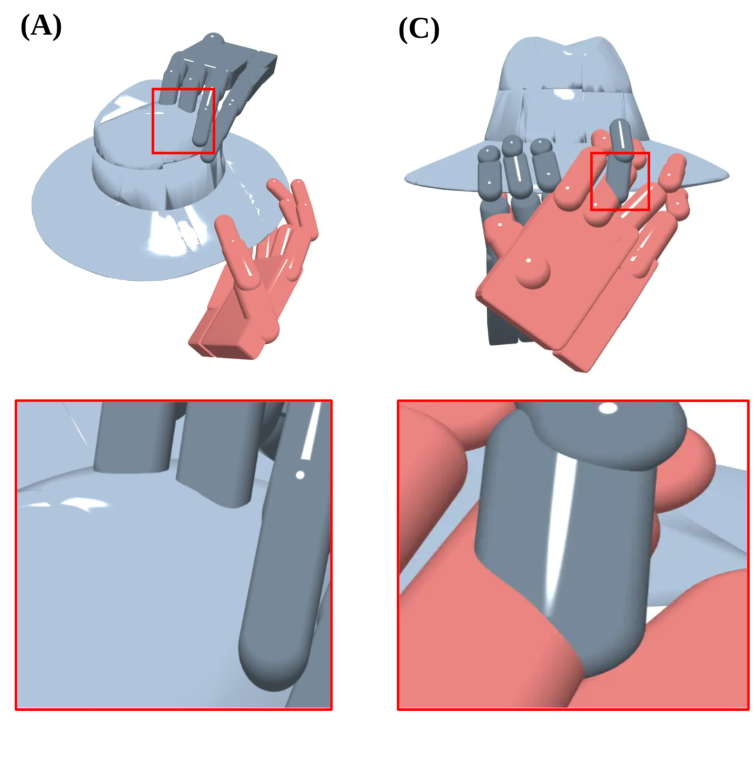
\includegraphics[width=0.86\columnwidth]{figs/selected/bimanual_grasp_penetration.png}
    \caption{Two failures of synthesised two-hand grasps, each enlarged at the
      contact: (A) a finger inside the object, (C) a finger inside the other hand.
      Both look plausible whole~\cite{bimangrasp_2024}.}
    \label{fig:bimanual-penetration}
    \licensed[panels (A) and (C) of Fig.~9]{Fig.~9 of Shao and Xiao, arXiv:2411.15903}{CC BY 4.0}{https://creativecommons.org/licenses/by/4.0/}
  \end{figure}}
}{}}{}
\makeatother

A dexterous policy is defined by what supervises it, and four sources are in use across the
corpus's 112 method rows: a reward function supervises reinforcement learning, a human
demonstration supervises imitation, a human reference trajectory supervises a physics-based
tracker, which is imitation with a simulator in the loop, and nothing supervises a model-based
planner, which is handed a cost and a model instead.

The labels do not partition the corpus. Of the 112 method rows, 53 are tagged reinforcement
learning, 27 behaviour cloning, 23 distillation, 18 generalist or vision-language-action, 14
teleoperation systems, 14 diffusion, 10 data collection, 8 flow matching, 6 reinforcement learning
from demonstrations, 6 trajectory optimisation, 5 model-predictive control, 4 grasp synthesis and
2 world models. The tags sum to far more than 112 because most methods published since 2024 sit on
two branches at once. \figurename~\ref{fig:taxonomy} draws the tree and the cross-links. The
repository carries the row-by-row version of the same thing, one row per method, and that is what
to scan when looking for work comparable to your own.

What the deployed policy looks like once training is done matters more than the name a paper gives
itself, and on that axis the field has converged hard. Section~\ref{sec:train:hybrids} shows why.

\textbf{What the tabulation does not record.}\label{sec:train:master}
The emptiest columns of the method tabulation are the ones a reader most needs: only 31 rows state
an environment count, only 70 state how many real trials are behind the headline number, and only
39 state how many unseen objects were tested. The trial and unseen-object figures are the audited
ones, after Section~\ref{subsec:reporting} recovered 15 trial counts and 7 unseen-object counts that
the notes carried and the extraction had dropped. A mostly empty row is not a weak method, but it is
one that cannot be compared with any other row here. All 112 rows carry the columns this survey
reads, and Appendix~\ref{app:method} says where they are and how to read them.

\begin{figure*}[!t]
  \centering
  \IfFileExists{figs/fig_taxonomy.tex}{% Figure: what supervises a dexterous policy. Drawn for the LaTeX edition in the restrained
% palette: greyscale plus the one accent, thin rules, square corners, document font. It redraws
% paper/figures/fig4_taxonomy.svg to the specification carried in paper/sections/05_training.md.
% Every count is the number of corpus method rows the leaf's stated predicate selects, recomputed
% from corpus/rows/*.json with the predicates of tools/make_flow_tree.py, so no leaf claims more
% than it tests: the PPO leaves read `algorithm` and `sim` rather than the RL tag, the reward
% branch counts RL and RL+demo together, the demonstration branch counts the union of BC,
% diffusion and flow, and the no-learning branch counts the three papers that learn no policy
% rather than the eleven rows carrying a trajopt or MPC tag. A paper may appear at more than one
% leaf. Bars are linear in the count. Designed for a two-column figure* at 18.1 cm.
\begin{tikzpicture}[
  font=\footnotesize,
  bar/.style={draw=none,fill=black!62},
  baracc/.style={draw=none,fill=accent},
  box/.style={draw=black!45,line width=0.3pt,inner sep=3pt,align=left},
  tree/.style={draw=black!45,line width=0.35pt},
  lnk/.style={draw=black!38,line width=0.28pt},
  lbl/.style={font=\scriptsize,anchor=west},
  ann/.style={font=\scriptsize\itshape,anchor=west},
  key/.style={font=\scriptsize\ttfamily\color{black!58},anchor=west},
  num/.style={font=\scriptsize,anchor=west},
  bname/.style={font=\scriptsize\bfseries,anchor=north west,align=left,text width=2.7cm},
  xl/.style={draw=black!45,line width=0.3pt,dash pattern=on 2pt off 1.6pt,-latex},
  xt/.style={draw=accent,line width=0.4pt,dash pattern=on 3pt off 1.4pt on 1pt off 1.4pt,-latex},
  xw/.style={font=\tiny\itshape\color{black!58},fill=white,inner sep=0.6pt},
  ftr/.style={font=\scriptsize,anchor=north west,align=left,text width=17.6cm},
]
\node[box,anchor=west,text width=2.0cm] (root) at (0,-6.48) {\scriptsize\textbf{supervision for a dexterous policy}\\[1pt]{\tiny 112 method papers}};
\draw[box] (2.90,0.22) rectangle (6.40,-2.92);
\node[bname] at (3.02,0.16) {a reward function};
\node[num,anchor=east,font=\scriptsize\bfseries] at (6.28,0.03) {59};
\node[anchor=east,font=\tiny\color{black!55}] at (6.28,-0.23) {41 of 59 in a leaf};
\draw[tree] (root.east) .. controls (2.55,-6.48) and (2.65,-1.35) .. (2.90,-1.35);
\draw[tree] (6.55,0.00) -- (6.55,-2.70);
\draw[tree] (6.40,-1.35) -- (6.55,-1.35);
\draw[tree] (6.55,0.00) -- (6.69,0.00);
\draw[tree] (6.55,-1.08) -- (6.69,-1.08);
\draw[tree] (6.55,-2.16) -- (6.69,-2.16);
\draw[tree] (6.55,-2.70) -- (6.69,-2.70);
\draw[box] (2.90,-3.38) rectangle (6.40,-7.60);
\node[bname] at (3.02,-3.44) {a human demonstration};
\node[num,anchor=east,font=\scriptsize\bfseries] at (6.28,-3.57) {44};
\node[anchor=east,font=\tiny\color{black!55}] at (6.28,-3.83) {26 of 44 in a leaf};
\draw[tree] (root.east) .. controls (2.55,-6.48) and (2.65,-5.49) .. (2.90,-5.49);
\draw[tree] (6.55,-3.60) -- (6.55,-5.22);
\draw[tree] (6.40,-5.49) -- (6.55,-5.49);
\draw[tree] (6.55,-3.60) -- (6.69,-3.60);
\draw[tree] (6.55,-4.14) -- (6.69,-4.14);
\draw[tree] (6.55,-4.68) -- (6.69,-4.68);
\draw[tree] (6.55,-5.22) -- (6.69,-5.22);
\draw[box] (2.90,-8.06) rectangle (6.40,-11.20);
\node[bname] at (3.02,-8.12) {a human reference, tracked with physics};
\node[num,anchor=east,font=\scriptsize\bfseries] at (6.28,-8.25) {12};
\draw[tree] (root.east) .. controls (2.55,-6.48) and (2.65,-9.63) .. (2.90,-9.63);
\draw[tree] (6.55,-8.28) -- (6.55,-10.98);
\draw[tree] (6.40,-9.63) -- (6.55,-9.63);
\draw[tree] (6.55,-8.28) -- (6.69,-8.28);
\draw[tree] (6.55,-8.82) -- (6.69,-8.82);
\draw[tree] (6.55,-9.36) -- (6.69,-9.36);
\draw[tree] (6.55,-9.90) -- (6.69,-9.90);
\draw[tree] (6.55,-10.44) -- (6.69,-10.44);
\draw[tree] (6.55,-10.98) -- (6.69,-10.98);
\draw[box] (2.90,-11.66) rectangle (6.40,-13.18);
\node[bname] at (3.02,-11.72) {no learned policy};
\node[num,anchor=east,font=\scriptsize\bfseries] at (6.28,-11.85) {3};
\draw[tree] (root.east) .. controls (2.55,-6.48) and (2.65,-12.42) .. (2.90,-12.42);
\draw[tree] (6.55,-11.88) -- (6.55,-12.96);
\draw[tree] (6.40,-12.42) -- (6.55,-12.42);
\draw[tree] (6.55,-11.88) -- (6.69,-11.88);
\draw[tree] (6.55,-12.42) -- (6.69,-12.42);
\draw[tree] (6.55,-12.96) -- (6.69,-12.96);
\fill[bar] (6.75,-0.06) rectangle (7.75,0.06);
\node[num] at (7.85,0.00) {20};
\node[lbl] at (8.45,0.09) {PPO in a GPU-parallel simulator, no distillation stage};
\node[key] at (8.45,-0.15) {physhoi\_2023, force\_grasp\_sim2real\_2026, and 18 more};
\fill[baracc] (6.75,-0.60) rectangle (6.80,-0.49);
\node[num] at (7.85,-0.54) {1};
\node[ann] at (8.79,-0.45) {-- population-based training over hyperparameters};
\node[key] at (8.79,-0.69) {dexpbt\_2023};
\fill[bar] (6.75,-1.14) rectangle (7.55,-1.03);
\node[num] at (7.85,-1.08) {16};
\node[lbl] at (8.45,-0.99) {plus teacher-student distillation};
\node[key] at (8.45,-1.23) {unidexgrasp\_2023, dexplore\_2025, and 14 more};
\fill[bar] (6.75,-1.68) rectangle (7.00,-1.57);
\node[num] at (7.85,-1.62) {5};
\node[ann] at (8.79,-1.53) {-- of which the student is a vision policy};
\node[key] at (8.79,-1.77) {hora\_2022, visual\_dexterity\_2022, and 3 more};
\fill[baracc] (6.75,-2.22) rectangle (6.85,-2.10);
\node[num] at (7.85,-2.16) {2};
\node[lbl] at (8.45,-2.07) {reward written by a language model};
\node[key] at (8.45,-2.31) {eureka\_2023, dreureka\_2024};
\fill[bar] (6.75,-2.76) rectangle (7.05,-2.65);
\node[num] at (7.85,-2.70) {6};
\node[lbl] at (8.45,-2.61) {seeded by demonstrations (the RL+demo tag)};
\node[key] at (8.45,-2.85) {pianomime\_2024, dexmv\_2021, and 4 more};
\fill[bar] (6.75,-3.66) rectangle (7.45,-3.54);
\node[num] at (7.85,-3.60) {14};
\node[lbl] at (8.45,-3.51) {teleoperated on the target robot};
\node[key] at (8.45,-3.75) {dexteleop0\_2026, dexora\_2026, and 12 more};
\fill[bar] (6.75,-4.20) rectangle (6.95,-4.09);
\node[num] at (7.85,-4.14) {4};
\node[lbl] at (8.45,-4.05) {wearable or hand-held rig, no robot in the loop};
\node[key] at (8.45,-4.29) {dexcap\_2024, dexumi\_2025, and 2 more};
\fill[bar] (6.75,-4.74) rectangle (7.10,-4.63);
\node[num] at (7.85,-4.68) {7};
\node[lbl] at (8.45,-4.59) {egocentric video, no robot at all};
\node[key] at (8.45,-4.83) {dexmv\_2021, videodex\_2022, and 5 more};
\fill[baracc] (6.75,-5.28) rectangle (6.85,-5.17);
\node[num] at (7.85,-5.22) {2};
\node[lbl] at (8.45,-5.13) {synthetic demonstration generation};
\node[key] at (8.45,-5.37) {dexmimicgen\_2024, deximit\_2026};
\fill[baracc] (6.75,-5.82) rectangle (6.80,-5.71);
\node[num] at (7.85,-5.76) {1};
\node[ann] at (8.79,-5.67) {-- policy shape, an independent choice: action chunking};
\node[key] at (8.79,-5.91) {aloha\_act\_2023};
\fill[bar] (6.75,-6.36) rectangle (7.45,-6.25);
\node[num] at (7.85,-6.30) {14};
\node[ann] at (8.79,-6.21) {-- diffusion};
\node[key] at (8.79,-6.45) {diffusion\_policy\_2023, dp3\_2024, and 12 more};
\fill[bar] (6.75,-6.90) rectangle (7.15,-6.79);
\node[num] at (7.85,-6.84) {8};
\node[ann] at (8.79,-6.75) {-- flow matching};
\node[key] at (8.79,-6.99) {pi0\_2024, groot\_n1\_2025, and 6 more};
\fill[baracc] (6.75,-7.44) rectangle (6.85,-7.33);
\node[num] at (7.85,-7.38) {2};
\node[ann] at (8.79,-7.29) {-- autoregressive action tokens};
\node[key] at (8.79,-7.53) {openvla\_2024, metis\_2025};
\fill[bar] (6.75,-8.34) rectangle (6.95,-8.23);
\node[num] at (7.85,-8.28) {4};
\node[lbl] at (8.45,-8.19) {whole reference including fingers};
\node[key] at (8.45,-8.43) {dextrack\_2025, maniptrans\_2025, and 2 more};
\fill[baracc] (6.75,-8.88) rectangle (6.80,-8.77);
\node[num] at (7.85,-8.82) {1};
\node[lbl] at (8.45,-8.73) {wrist only, fingers learned};
\node[key] at (8.45,-8.97) {objdex\_2024};
\fill[baracc] (6.75,-9.41) rectangle (6.80,-9.30);
\node[num] at (7.85,-9.36) {1};
\node[lbl] at (8.45,-9.27) {object trajectory only};
\node[key] at (8.45,-9.51) {human2sim2robot\_2025};
\fill[baracc] (6.75,-9.95) rectangle (6.80,-9.84);
\node[num] at (7.85,-9.90) {1};
\node[lbl] at (8.45,-9.81) {reference as soft guidance};
\node[key] at (8.45,-10.05) {dexplore\_2025};
\fill[baracc] (6.75,-10.49) rectangle (6.85,-10.38);
\node[num] at (7.85,-10.44) {2};
\node[lbl] at (8.45,-10.35) {no retargeting, reference already on the embodiment};
\node[key] at (8.45,-10.59) {physhoi\_2023, omnigrasp\_2024};
\fill[baracc] (6.75,-11.03) rectangle (6.90,-10.92);
\node[num] at (7.85,-10.98) {3};
\node[lbl] at (8.45,-10.89) {whole-body humanoid, hands carried with the body};
\node[key] at (8.45,-11.13) {dexman\_2025, humanplus\_2024, omnih2o\_2024};
\fill[baracc] (6.75,-11.93) rectangle (6.80,-11.82);
\node[num] at (7.85,-11.88) {1};
\node[lbl] at (8.45,-11.79) {sampled plan, learned model};
\node[key] at (8.45,-12.03) {pddm\_2019};
\fill[baracc] (6.75,-12.47) rectangle (6.80,-12.36);
\node[num] at (7.85,-12.42) {1};
\node[lbl] at (8.45,-12.33) {sampled plan, given model};
\node[key] at (8.45,-12.57) {mjpc\_2022};
\fill[baracc] (6.75,-13.01) rectangle (6.80,-12.90);
\node[num] at (7.85,-12.96) {1};
\node[lbl] at (8.45,-12.87) {smoothed analytic contact model};
\node[key] at (8.45,-13.11) {pang\_global\_planning\_2022};
\draw[xl] (16.20,-1.08) .. controls (16.55,-1.08) and (16.55,-5.49) .. (16.20,-5.49);
\node[xw] at (16.57,-3.29) {distil};
\draw[xl] (16.20,0.00) .. controls (16.82,0.00) and (16.82,-5.22) .. (16.20,-5.22);
\node[xw] at (16.84,-2.61) {generate};
\draw[xl] (16.20,-4.68) .. controls (17.09,-4.68) and (17.09,-9.63) .. (16.20,-9.63);
\node[xw] at (17.11,-7.15) {retarget};
\draw[xl] (16.20,-9.63) .. controls (17.36,-9.63) and (17.36,-5.49) .. (16.20,-5.49);
\node[xw] at (17.38,-7.56) {distil};
\draw[xt] (16.20,-12.42) .. controls (17.63,-12.42) and (17.63,0.00) .. (16.20,0.00);
\node[xw] at (17.65,-6.21) {smooth};
\draw[xl] (16.20,-3.60) .. controls (17.90,-3.60) and (17.90,-2.70) .. (16.20,-2.70);
\node[xw] at (17.92,-3.15) {seed};
\node[ftr] at (0,-13.80) {Eight further rows carry a trajectory-optimisation or MPC tag inside a learned pipeline and are counted on the branch that learns. The double-dashed edge is the one overlap that is a theorem rather than a pipeline: \texttt{pang\_global\_planning\_2022} proves that a policy gradient and an analytic log-barrier relaxation compute the same local model of contact.};
\end{tikzpicture}
}{%
    \framebox[0.7\textwidth]{\rule{0pt}{2.2cm}\textit{figs/fig\_taxonomy.tex pending}}}
  \caption{What supervises a dexterous policy, subdivided to where the 112 method papers actually
  differ; each leaf is keyed to the corpus, bars scaled by row count, dashed curves marking
  overlap.}
  \label{fig:taxonomy}
\end{figure*}

\subsection{Reinforcement learning}
\label{sec:train:rl}

\textbf{The standard recipe.}\label{sec:train:rl:recipe}
Fifty-nine of the 112 method rows learn from a reward. Forty-eight name PPO as the algorithm, and
the next most frequent, DAPG, appears four times. Forty-three run their own experiments in a
GPU-parallel simulator from the Isaac family or Genesis, and 36 do both. Only 31 rows state an
environment count, with a median of 8192 and a maximum of 64000. Twenty-three rows distil a
privileged teacher into a deployable student, and 16 combine all three of PPO, a GPU simulator and
distillation. That 16-row intersection is the recipe as it is actually practised.

The hand is almost always an Allegro. It appears in 35 of the 112 method rows and in 17 of the 31
reorientation rows, ahead of Shadow at 21 and 6 and LEAP at 12 and 4.

Privilege is handled two ways. OpenAI \cite{openai_dexterity_2018} gives the value network object
and target orientation, joint angles, joint velocities and object velocities the policy never
sees, with a footnote recording that current object orientation was left out of the policy inputs
by accident, and DeXtreme \cite{dextreme_2022} uses the same asymmetric critic with a 2048-unit
LSTM against the actor's 1024. Hora \cite{hora_2022} instead compresses nine privileged object
properties into an eight-dimensional vector regressed from 30 steps of proprioception, and Visual
Dexterity \cite{visual_dexterity_2022} distils twice, from a state teacher to a synthetic point
cloud and then to a rendered one, for a fivefold speedup.

Domain randomisation is the part of the recipe with the least discipline. OpenAI
\cite{openai_rubiks_cube_2019} made it adaptive, pushing each range boundary out when performance
at that boundary exceeds 20 successes and pulling it in below 10, and DeXtreme
\cite{dextreme_2022} reproduced the mechanism with a 256-sample queue and 40 percent of
environments dedicated to boundary evaluation. Both publish the discovered ranges. Below that
standard, two shipped configurations disagree with their own papers about what was randomised:
Hora \cite{hora_2022} states a joint-noise range of U(0, 0.005) against a shipped
\texttt{jointNoiseScale} of 0.02, in a commit its own README says is not the one that reproduces
the paper, and PenSpin \cite{penspin_2024} zeroes the disturbance force its appendix describes.
DexPBT \cite{dexpbt_2023}'s \texttt{randomize: False} is not a third case: it is the IsaacGymEnvs
default and agrees with the paper's statement that randomisation was not used here.

\textbf{Reward engineering.}\label{sec:train:rl:reward}
The repository puts the 21 in-hand reorientation methods against nine recurring term families and
marks each cell by where the term was found: in the paper, in the code, in both, or in the code
with every shipped configuration setting its weight to zero.

% The matrix itself is not set here. It is a lookup table over 21 methods and nine term
% families, and it is in the repository: \texttt{corpus/reward\_matrix.json} and
% \texttt{paper/tables/table5\_rewards.md}. Every mark this subsection reads out is named in
% the prose below rather than pointed at.

The families are not equally popular. Nineteen of 21 methods have a goal or rotation tracking
term, which is the task. Thirteen penalise effort as torque, work or joint velocity, 13 pay a
sparse success bonus, 11 penalise object velocity and 10 penalise a drop. Eight penalise deviation
of the hand from a canonical grasp pose, a family the plan for that matrix did not anticipate and
which had to be added. Six penalise action rate or magnitude, five reward closing the distance
from fingertips to the object, and four carry a contact or force mark at all.

Three marks an earlier draft recorded as \emph{code} now read \emph{code (0)}, because in each the
term is in the released code with every shipped configuration setting its weight to zero: DeXtreme
\cite{dextreme_2022}'s timeout reward, DexPBT \cite{dexpbt_2023}'s fall penalty, and PenSpin
\cite{penspin_2024}'s action penalty. Marking them \emph{code} would tell a reader the code
optimises something the paper does not state, and leaving them unmarked would hide a term that is
in the file. The repository carries the config key and the zero beside each of the three marks.

Only three of the four contact marks are the finding. AnyRotate \cite{anyrotate_2024} scores good
and bad fingertip contacts, Lin et al. \cite{poise_2026} reward a friction-cone wrench margin, and
Zhao et al. \cite{force_grasp_sim2real_2026} track a commanded grasp force. The fourth,
\cite{visual_dexterity_2022}, penalises the \emph{object} touching the table, a task-shaping term
against using the table as a third finger rather than a hand-object term, and its table-contact
flag defaults to off, with no shipped config setting it true. Three of 21 in-hand reorientation
methods, then, put a hand-object contact or force quantity in the reward, and none puts
interpenetration in it. Li et al. \cite{teledexter_2026} penalise interpenetration with a
differentiable signed-distance term, but during offline reference construction, not in the
policy's reward. Across all 112 method rows, 85 do not address penetration at all, 5 constrain it,
3 measure it, 3 penalise it and 16 say nothing either way. The physical quality of the contact is
not something this literature optimises.

Term counts range from one to ten. DemoStart \cite{demostart_2024} gives a single binary terminal
reward of 1 and lets a curriculum over demonstration states do the shaping. AnyRotate
\cite{anyrotate_2024} and ViserDex \cite{viserdex_2026} each publish ten weighted terms. ViserDex
is the cleanest specification of the 21, with every term, weight and equation in one appendix
table, and a statement that the same weights are used for every object.

Weights are frequently unrecoverable. Three of the 21 rows give no numeric weight that survives
PDF conversion, because the equation blocks are images, which is a limit of this survey and is
recorded as such. Robot Synesthesia \cite{robot_synesthesia_2023} is a worse case. Its six
coefficients are described only as ``tuned hyper-parameters'' and no number is printed anywhere in
the paper, so the reward it reports cannot be reconstructed by anyone. DexReMoE
\cite{dexremoe_2025} names an angular-velocity penalty weight in prose with no entry in its
hyperparameter table, and DexTrack \cite{dextrack_2025} names an affinity reward that is missing
from its weight table.

\textbf{Curricula, populations and machine-written rewards.}\label{sec:train:rl:curricula}
Curricula in this literature relax physics or tighten tolerances. DexPBT \cite{dexpbt_2023}
tightens a success tolerance from 0.075 to 0.01 by a factor of 0.9 every 3000 environment steps
once three successes are logged, and ManipTrans \cite{maniptrans_2025} starts at zero gravity and
high friction and restores both while narrowing a fingertip threshold from 6 cm to 4 cm.
DexMachina \cite{dexmachina_2025} attaches virtual spring-damper controllers to the object, lets
them do the task at first, then decays their gains to zero. The two that ablate the curriculum
report it is load-bearing: RotateIt \cite{rotateit_2023} sets its rotation-penalty weight to zero
and ramps it to $-0.1$, because applying it from the start makes the policy learn only to hold the
object still, and ViserDex \cite{viserdex_2026}, whose performance-based curriculum runs over
regularisation weight, action latency and time between successes, fails completely without the
regularisation component.

Population-based training appears once. DexPBT \cite{dexpbt_2023} runs populations of 8, 16 and 32
agents, splits them 30/40/30, mutates the middle and replaces the bottom with mutated copies of
the top, each float hyperparameter multiplied or divided by a factor drawn from U(1.1, 1.5) with
probability 0.2. It reports 30 hours on a single V100 for a five-billion-transition single-arm
run, and 0.32 trillion environment steps for its largest population.

Eureka \cite{eureka_2023} has GPT-4 write the reward function directly, constrained to return a
total and a dictionary of named components, and feeds per-component statistics back between
iterations. Its appendix gives an example whose reward correlates at $-0.26$ with the
human-written one and still scores 1.45 on the human-normalised metric, the strongest argument in
the corpus that hand-tuned weights are not a ceiling. DrEureka \cite{dreureka_2024} moves the
safety requirement into the prompt instead of a penalty term, asking in words for a cube rotating
at about 0.25 radians per second with fingers penalised for leaving their initial pose. Neither
can be checked against a file. Eureka's generated rewards are written at run time to a gitignored
directory and never committed, so the reward behind any reported number cannot be recovered from
the repository, though its README documents the paper's budget of five iterations and sixteen
samples as the default and marks the shipped one-iteration block a fast-test preset. DrEureka's
repository contains only the locomotion and globe-walking trees, so its LEAP-hand reward has no
code at all.

\textbf{Where reinforcement learning stalls.}\label{sec:train:rl:stalls}
Reinforcement learning stalls on objectives that are not learnable as stated. AnyRotate
\cite{anyrotate_2024} found the angular-velocity objective unlearnable in the multi-axis setting
and replaced it with a moving keypoint target. RotateIt \cite{rotateit_2023} reports that its
multi-axis policy ``does not converge when training with only reinforcement learning'' and adds an
imitation loss against single-axis oracles. Eureka \cite{eureka_2023} cannot spin a pen from
scratch and needs a pretrain-then-finetune split, with the from-scratch ablation failing to
complete one cycle. Section~\ref{sec:train:track}'s contact-graph term exists because of the general shape of the
problem: contact moves the object off the reference, so return goes down, so the policy learns not
to touch the object.

It stalls on geometry too. Hora \cite{hora_2022} fails on objects under 4 cm across because the
fingers collide with each other. What it does not stall on is publication: the real-trial counts
behind these headlines are small enough that Section~\ref{subsec:reporting} treats them as the reporting problem
they are.

\subsection{Learning from human data}
\label{sec:train:human}

\textbf{Teleoperation and retargeting.}\label{sec:train:human:teleop}
Thirty corpus rows describe a system for getting human motion onto a robot hand; the repository
lists them with the retargeting objective compressed to one clause each.

% The 30 systems are a lookup table from beginning to end, so they are tabulated in the
% repository rather than set here: \texttt{paper/tables/table6\_teleop.md}.

Retargeting splits four ways. The dominant family matches task-space vectors between the human and
robot hands. DexPilot \cite{dexpilot_2020} set the pattern with a weighted squared distance
between fingertip vectors, switching weights of 1, 200 and 400 by whether a pair is within
threshold, a minimum-separation constant of 3 cm between primary fingers, and a regulariser toward
the open hand, solved online with SLSQP; AnyTeleop \cite{anyteleop_2023}, Open-TeleVision
\cite{open_television_2024}, Bunny-VisionPro \cite{bunny_visionpro_2024} and ACE
\cite{ace_teleop_2024} all use the same formulation. The second copies joint angles where the
kinematics allow it, as Holo-Dex \cite{holo_dex_2022} does for index, middle and ring while
solving the thumb by inverse kinematics and discarding the pinky the Allegro does not have. The
third learns the map offline: Geometric Retargeting \cite{geometric_retargeting_2025} trains a
per-finger network in three to five minutes against motion-direction, coverage, flatness, pinch
and collision criteria, then runs at 1 kHz against the 60 to 100 Hz of online optimisation,
raising configuration-space coverage from 38 to 90 percent and one-time grasp success from 55 to
87.5 percent. The fourth removes retargeting from the loop: DexUMI \cite{dexumi_2025} builds an
exoskeleton whose fingertip workspace is optimised to match the target hand, then regresses
encoder values straight to motor values.

What that tabulation does not carry is the point. Only 12 of the 30 rows record a latency at all,
three of those give no number, and only 7 state a rig cost. Where costs are stated they are low
and falling, from \cite{holo_dex_2022}'s \$399 headset through the \$600 exoskeleton of
\cite{ace_teleop_2024} and the \$600 haptic glove of \cite{doglove_2025} to the \$4,000 backpack
of \cite{dexcap_2024} and the \$6,000 rig of \cite{bidex_teleop_2024}. Latency is not one
quantity: DexPilot \cite{dexpilot_2020}'s ``about one second'' and Holo-Dex \cite{holo_dex_2022}'s
``under 100 milliseconds'' are end to end, while Geometric Retargeting
\cite{geometric_retargeting_2025}'s 1 kHz and AnyTeleop \cite{anyteleop_2023}'s 9 to 10 ms
retargeting are single stages and several cells give a control rate. That tabulation's latency
column mixes the two, so its spread is not a range. Only 13 rows report how many trajectories were
collected, and only 7 report hours.

Where throughput is measured, human collection beats teleoperation by a wide margin. Qiu et al.
\cite{humanoid_policy_human_policy_2025} time a grasp demonstration at 3.79 seconds for a bare
human and 19.72 seconds through a teleoperated humanoid, and a pour at 4.81 against 37.31 seconds.
It attributes the gap to retargeting latency and to the workspace of a 7-DoF arm rather than to
anything about the hand.

\textbf{Imitation architectures.}\label{sec:train:human:arch}
Four architectures cover the corpus. Action chunking came from \cite{aloha_act_2023}, which
predicts a chunk of joint targets with a CVAE and combines overlapping chunks by exponentially
weighted ensembling, reaching 80 to 90 percent on fine bimanual tasks from about 50 demonstrations
each. Diffusion came from Diffusion Policy \cite{diffusion_policy_2023}, which denoises an action
sequence and reports a 46.9 percent average success improvement over LSTM-GMM, IBC and BET across
15 tasks. 3D Diffusion Policy \cite{dp3_2024} swaps the image encoder for a small point-cloud
encoder and reports 74.4 percent against 59.8 percent across 72 simulated tasks, and 85.0 against
35.0 percent on four real tasks from 40 demonstrations each. Flow matching is the 2024-onward
default for large models and carries 8 of the 112 rows. Discrete action tokens are the fourth,
used by \cite{openvla_2024} and \cite{metis_2025}, and are the only one of the four that needs no
continuous head at all.

Data generation is a separate lever and is underrated. DexMimicGen \cite{dexmimicgen_2024} turns
60 human source demonstrations into 21,000 simulated ones across 9 tasks and 3 embodiments, and a
real Fourier GR1 with two Inspire hands reaches 90 percent from 40 generated demonstrations
against 0 percent from the 4 source ones. Dex1B \cite{dex1b_2025} iterates optimisation, a CVAE
proposal model and a simulator filter into roughly a billion synthetic grasps, and its CVAE
baseline beats the prior best by 22 points.

\textbf{Human video without a robot.}\label{sec:train:human:video}
Seven rows train a dexterous-hand policy from video with no teleoperation at any stage. DexMV
\cite{dexmv_2021} retargets 700 self-recorded demonstrations by matching palm-to-fingertip
task-space vectors and estimating actions by inverse dynamics, VideoDex \cite{videodex_2022} mines
965 trajectories from EpicKitchens to pretrain a neural dynamic policy, and DexVIP
\cite{dexvip_2022} goes further into the reward, clustering 715 curated HowTo100M frames into one
consensus grasp pose per object category and adding it as a reward term. OKAMI \cite{okami_2024},
Lum et al. \cite{human2sim2robot_2025} and Guzey et al. \cite{hudor_2024} work from a single video
each, and Goswami et al. \cite{wm_dex_human_videos_2025} pretrain a world model on 829 hours of
EgoDex.

\textbf{The embodiment gap.}\label{sec:train:human:gap}
Three papers measure the gap directly rather than asserting it. OKAMI \cite{okami_2024} runs the
same reference-plan and warping pipeline with and without human body and hand retargeting, and the
version without it loses 75.0, 42.1, 82.0 and 74.0 points across four task and setting pairs. That
is the largest clean embodiment-gap number in the corpus.

Qiu et al. \cite{humanoid_policy_human_policy_2025} ablate two mitigations separately on the same
vertical-grasp task over 10 trials. The full method scores 4 out of 10. Removing the interpolation
that slows human trajectories by a factor of four drops it to 1 out of 10. Removing the unified
54-dimensional state space while keeping the slowdown drops it to 0 out of 10, because the policy
is handed a shortcut for telling the two embodiments apart. EgoZero \cite{egozero_2025} reports
the sharpest version of the same effect. Removing 3D augmentation drops every one of its seven
tasks to 0 out of 15, and substituting monocular depth for triangulated depth does the same,
because the best metric depth models it tested carry more than 5 cm of error. It also quantifies
what its hand-pose pipeline costs, at 1 to 2 cm of action-label error.

Chen et al. \cite{objdex_2024} supply the counterexample. Their method retargets only the wrist
and lets reinforcement learning discover finger motion, and their ablation that adds a
fingertip-matching reward ``does not yield benefits and even leads to lower performance''. Richer
human correspondence is not uniformly better, and this is the one result in the corpus that says
so with an ablation.

\textbf{Tracking a human reference with physics.}\label{sec:train:track}
Twelve method rows sit in the human-reference tracking family. Eight track a human hand on an
object and are covered here; the other four sit at the edges, Lum et al.
\cite{human2sim2robot_2025} tracking only the object's trajectory, DexMan \cite{dexman_2025}
retargeting bimanual video onto a full humanoid, and HumanPlus \cite{humanplus_2024} and OmniH2O
\cite{omnih2o_2024} tracking whole-body motion. A reference is retargeted onto the robot and a
policy trained to make the simulated body follow it: the reference supplies the shaping reward
engineering would otherwise have to invent, and the simulator the physical consistency pure
imitation lacks.

PhysHOI \cite{physhoi_2023} is the origin of the reward form. It multiplies a body term, an object
term, an interaction-graph term and a contact-graph term, and reaches 95.4 percent success on GRAB
against 27.0 percent for a DeepMimic baseline. The contact-graph term exists to stop the policy
learning not to touch the object. Omnigrasp \cite{omnigrasp_2024} replaces the action space with a
pretrained latent motion prior and reports 94.6 percent grasp success and 84.8 percent trajectory
success on GRAB, while stating outright that it omits penetration metrics.

DexTrack \cite{dextrack_2025} adds an imitation loss to PPO and mines its own demonstrations
through a homotopy search over easier neighbouring trajectories, reaching 46.70 and 65.48 percent
on GRAB at loose and strict thresholds against 38.58 and 54.82 for the best baseline. It has a
penetration-depth formula and applies it only to input references, never to its own rollouts, and
presents tolerance of ``severe hand-object penetrations'' as robustness. ManipTrans
\cite{maniptrans_2025} freezes a generalist hand imitator and trains a per-task residual on top,
reaching 58.1 percent single-hand and 39.5 percent bimanual success on OakInk-V2. Its stance on
contact is to raise the friction coefficient above the real value rather than model skin
deformation, and its real deployment is open-loop replay.

DexMachina \cite{dexmachina_2025} moves to Genesis with 12,000 environments and six hand URDFs,
and drives the object with virtual controllers that decay to zero. Its re-implementation of
\cite{maniptrans_2025}'s curriculum does not beat no curriculum on its own setup, which is a
direct disagreement between two papers worth quoting in both directions. Dexplore
\cite{dexplore_2025} drops the explicit retargeting stage and treats the reference as soft
guidance, with termination thresholds derived from the failure rate, reaching 87.7 percent on GRAB
with an Inspire hand.

% What retargeting gets wrong, at the contact set.
\providecommand{\plateRetargetArtifacts}{}\plateRetargetArtifacts

TopoRetarget \cite{toporetarget_2026} is the only corpus method that quantifies penetration as an
evaluation quantity, reporting maximum depth and the fraction of frames past 2 mm, and
constraining it during retargeting with a 1 mm soft tolerance and a 30 mm hard bound. It reaches
87.5 percent on its own pen-spinning set against 46.9 for the best baseline. It does not
re-measure penetration after the tracking policy runs, so the property it constrains is a property
of the reference and not of the behaviour. \figurename~\ref{fig:teleop-retarget-artifacts} is what
that property looks like when it is not held: the pose is plausible and the contact is not.

That is the pattern across all eight, and it is the reference-versus-rollout split in its sharpest
form. Penetration is handled at the reference, if at all, and never at the rollout. Chen et al.
\cite{objdex_2024} complete the set with the only real-robot numbers among them, from 100 percent
on a microwave and a laptop down to 41.2 percent on a ketchup bottle over 20 trials each.

\textbf{The retargeting map, and what would close it.} Human data does not port across hands, and
the map is usually left unstated. Fifty-three method rows use human data and name 45 distinct hand
strings between them, and twenty of those appear among the 30 teleoperation systems with a stated
retargeting objective. The other 33 never say how the human motion reached the hand, and the stated
objectives do not converge, from a fingertip keypoint-vector energy in \cite{anyteleop_2023} to a
per-joint regression from exoskeleton encoders in \cite{dexumi_2025} to no retargeting at all in
\cite{egozero_2025}. What would close it is a retargeting benchmark in TopoRetarget's form
\cite{toporetarget_2026}, reporting contact precision, contact alignment, maximum penetration and
the share of frames past 2 mm, per hand and per dataset.

\subsection{Generalist and vision-language-action policies}
\label{sec:train:vla}

The finding is the size of the hand. Eighteen rows carry the generalist tag. Fourteen of them
settle whether the reported evaluation ran on a multi-fingered hand. Eight of those fourteen did,
six report no hand result at all, and the remaining four never say, GR00T N1.6
\cite{groot_n16_2025} naming no end effector anywhere on its page.

Five of the eight state a hand size, and that comparison has to be made in actuated degrees of
freedom rather than joints, for the reason Section~III opens with. Four are six, the Inspire
RH56DFX among them actuating six of its twelve joints, and one is twelve, \cite{dexora_2026}'s
XHAND. Their median is 6. Two of the four rows that never settle the hand question do state a
size, and both are large: 21 for \cite{gr_dexter_2025}'s ByteDexter V2 and 22 for
\cite{egoscale_2026}'s Sharpa Wave. Of the 59 reward-learning rows, 48 state a count, 38 of those
are 16 or above, and their median is 16: an Allegro and a LEAP actuate 16, and a Shadow actuates
20 of its 24 joints. So no row that settles the question reaches the band the
reinforcement-learning literature of Section~\ref{sec:train:rl} works in, and the two rows that reach it on paper
are the two that never say whether the hand was in the evaluation. An earlier version of this
claim counted eleven rows as evaluating on a hand, which mixed the settled eight with rows the
notes leave open.

The six with no hand result are parallel-jaw throughout ($\pi_0$ \cite{pi0_2024}, whose released
code encodes each ALOHA gripper as one scalar, $\pi_{0.5}$ \cite{pi05_2025}, $\pi^{*}_{0.6}$
\cite{pistar06_2025}, OpenVLA \cite{openvla_2024}, Helix \cite{helix_2025}, which claims
individual-finger control of a 35-DoF upper body with no success rate or trial count for any task,
and Gemini Robotics \cite{gemini_robotics_2025}, whose Apollo hand appears in a figure caption
with no number attached). Its successor \cite{gemini_robotics_15_2025} closed that gap with Apollo
progress scores, not success rates, of 0.74 down to 0.62 across five generalisation axes. DexVLA
\cite{dexvla_2025} is the borderline case the other way: a hand in one real-robot task family,
grippers in the other five and in all 91 pretraining tasks.

The released code also drifts. GR00T N1 \cite{groot_n1_2025}'s repository is a later N1.7
generation with a different backbone, a different action horizon and embodiments the paper does
not describe, and the $\pi_{0.5}$ repository \cite{pi05_2025} supports only the flow-matching
head, not the hybrid recipe the paper describes.

\textbf{The size of the gap, and what would close it.} The gap is size rather than absence. The
generalist policies that do touch a hand run it at roughly a third of the actuation the
reinforcement-learning literature assumes, and the rows that never settle the question are the
smaller half of the same gap. What would close it is one dexterous-hand task in the standard
generalist suite, with the hand's actuated degrees of freedom and its vendor printed beside the
number.

\subsection{Model-based baselines and hybrids}
\label{sec:train:mbc}

Three corpus methods solve dexterous tasks without learning a policy, and they are the control
group the rest of this section lacks.

PDDM \cite{pddm_2019} learns an ensemble of dynamics models and plans through it with an
MPPI-style optimiser, replanning every step. It needs 1 to 2 hours of data in simulation and 2 to
4 hours on a real 24-DoF Shadow Hand. Predictive Sampling \cite{mjpc_2022} removes the learned
model too and samples ten rollouts per step through MuJoCo itself, planning in 1 to 20
milliseconds. It reorients a cube with a Shadow Hand in real time from scratch, and reports no
success criterion, no trial count and no real-robot result.

The work of Pang et al. \cite{pang_global_planning_2022} is the most substantial of the three. It
proves that the randomised smoothing implicit in reinforcement learning and an analytic
log-barrier relaxation compute the same local linear model of contact, then uses the analytic
version inside a trajectory optimiser and an RRT. Allegro in-hand rotation takes 19.59 seconds to
optimise and its plate-pickup task 117.16 seconds of planning on a 16-core CPU, against the
GPU-days of Section~\ref{sec:train:rl}, and it is the only method here that imposes non-penetration as a hard
constraint. Its own limitation is the honest part: its 3D systems transfer to hardware far worse
than its 2D ones, because the quasi-dynamic assumption breaks and planned grasps miss contacts
under a second-order solver.

\textbf{Hybrids, and where the field has converged.}\label{sec:train:hybrids}
The recurring shape is reinforcement learning in simulation distilled into a policy that looks
like an imitation policy, and it appears in four variants. The first distils a privileged teacher
into a vision student inside one paper, which is \cite{hora_2022}, \cite{visual_dexterity_2022},
\cite{rotateit_2023}, \cite{robot_synesthesia_2023} and \cite{viserdex_2026}. The second uses
reinforcement learning as a demonstration factory: DexTrack \cite{dextrack_2025} mines
demonstrations with per-trajectory RL and trains a generalist on them, ManipTrans
\cite{maniptrans_2025} does the same to build a 3.3K-episode dataset, and DexterityGen
\cite{dexteritygen_2025} trains a diffusion controller on ten billion simulated grasp-to-grasp
transitions and projects a human teleoperator's coarse command onto it, taking four reorientation
tasks from 0 out of 20 under raw teleoperation to 12, 13, 10 and 9 out of 20. The third generates
data without reinforcement learning at all, which is \cite{dexmimicgen_2024}, \cite{dex1b_2025}
and \cite{deximit_2026}; Dex1B's row is classed as a dataset, so \figurename~\ref{fig:taxonomy}'s
leaf, which counts method rows, holds the other two. The fourth wraps an RL policy in a residual,
which is \cite{resdex_2024} at 88.8 percent over 3,200 objects in 12 GPU-hours.

In the variants that dominate 2025 and 2026 work, the reward is no longer the objective of the
deployed policy. It is the objective of the process that produced the deployed policy's training
data. Reward engineering has moved upstream into data curation, and every reward-shaping pathology
in Section~\ref{sec:train:rl} now reaches the shipped policy through a dataset rather than a gradient.

\subsection{Paper against released code}
\label{sec:train:code}

% ---------------------------------------------------------------------------
% The first finding as a picture: the funnel from 112 method rows to the nine
% whose code contradicts the paper, with the 29 disagreements in the other four
% classes drawn at the same weight as the nine. Those 29 are classified, not
% retracted; the eight accusations the survey withdrew are counted in section
% 8.1 and in each accused row's mismatch_review field. Written by
% tools/make_finding_figures.py from corpus/rows; the guard keeps the document
% compiling until it is there. It sits in the subsection that argues the finding
% and classifies the 38, which is where a reader needs it.
% ---------------------------------------------------------------------------
\begin{figure}[!t]
  \centering
  \IfFileExists{figs/fig_codegap.tex}{\resizebox{\columnwidth}{!}{% generated by tools/make_finding_figures.py; do not edit
\begin{tikzpicture}[
  font=\footnotesize,
  bar/.style={draw=none,fill=black!62},
  barmid/.style={draw=none,fill=black!42},
  barlight/.style={draw=none,fill=black!20},
  baracc/.style={draw=none,fill=accent},
  seg/.style={draw=white,line width=0.5pt},
  lnk/.style={draw=black!38,line width=0.28pt},
  ghost/.style={draw=black!45,line width=0.3pt,dash pattern=on 1.2pt off 1.2pt},
  lbl/.style={font=\scriptsize},
  small/.style={font=\scriptsize\color{black!55}},
  num/.style={font=\scriptsize\color{black!55}},
]

\fill[barlight] (0.00,0.00) rectangle (4.90,-0.52);
\node[font=\small\bfseries\color{black!75}] at (2.45,-0.26) {112};
\node[lbl,anchor=west,align=left] at (5.20,-0.26) {method papers\\in the corpus};
\fill[black!7] (0.00,-0.52) -- (4.90,-0.52) -- (3.81,-0.78) -- (1.09,-0.78) -- cycle;
\fill[barmid] (1.09,-0.78) rectangle (3.81,-1.30);
\node[font=\small\bfseries\color{white}] at (2.45,-1.04) {62};
\node[lbl,anchor=west,align=left] at (5.20,-1.04) {released code that could\\be read against the paper};
\fill[black!7] (1.09,-1.30) -- (3.81,-1.30) -- (3.28,-1.56) -- (1.62,-1.56) -- cycle;
\fill[bar] (1.62,-1.56) rectangle (3.28,-2.08);
\node[font=\small\bfseries\color{white}] at (2.45,-1.82) {38};
\node[lbl,anchor=west,align=left] at (5.20,-1.82) {disagree with their\\own code somehow};
\fill[black!5] (1.62,-2.08) -- (3.28,-2.08) -- (7.60,-2.74) -- (0,-2.74) -- cycle;
\node[anchor=south east,font=\scriptsize\color{black!45}] at (7.60,-2.68) {one mark, one paper};
\fill[baracc] (0.00,-2.74) rectangle (0.15,-3.16);
\fill[baracc] (0.20,-2.74) rectangle (0.35,-3.16);
\fill[baracc] (0.40,-2.74) rectangle (0.55,-3.16);
\fill[baracc] (0.60,-2.74) rectangle (0.75,-3.16);
\fill[baracc] (0.80,-2.74) rectangle (0.95,-3.16);
\fill[baracc] (1.00,-2.74) rectangle (1.15,-3.16);
\fill[baracc] (1.20,-2.74) rectangle (1.35,-3.16);
\fill[baracc] (1.40,-2.74) rectangle (1.55,-3.16);
\fill[baracc] (1.60,-2.74) rectangle (1.75,-3.16);
\fill[barlight] (1.80,-2.74) rectangle (1.95,-3.16);
\fill[barlight] (2.00,-2.74) rectangle (2.15,-3.16);
\fill[barlight] (2.20,-2.74) rectangle (2.35,-3.16);
\fill[barlight] (2.40,-2.74) rectangle (2.55,-3.16);
\fill[barlight] (2.60,-2.74) rectangle (2.75,-3.16);
\fill[barlight] (2.80,-2.74) rectangle (2.95,-3.16);
\fill[barlight] (3.00,-2.74) rectangle (3.15,-3.16);
\fill[barlight] (3.20,-2.74) rectangle (3.35,-3.16);
\fill[barlight] (3.40,-2.74) rectangle (3.55,-3.16);
\fill[barlight] (3.60,-2.74) rectangle (3.75,-3.16);
\fill[barlight] (3.80,-2.74) rectangle (3.95,-3.16);
\fill[barlight] (4.00,-2.74) rectangle (4.15,-3.16);
\fill[barlight] (4.20,-2.74) rectangle (4.35,-3.16);
\fill[barlight] (4.40,-2.74) rectangle (4.55,-3.16);
\fill[barlight] (4.60,-2.74) rectangle (4.75,-3.16);
\fill[barlight] (4.80,-2.74) rectangle (4.95,-3.16);
\fill[barlight] (5.00,-2.74) rectangle (5.15,-3.16);
\fill[barlight] (5.20,-2.74) rectangle (5.35,-3.16);
\fill[barlight] (5.40,-2.74) rectangle (5.55,-3.16);
\fill[barlight] (5.60,-2.74) rectangle (5.75,-3.16);
\fill[barlight] (5.80,-2.74) rectangle (5.95,-3.16);
\fill[barlight] (6.00,-2.74) rectangle (6.15,-3.16);
\fill[barlight] (6.20,-2.74) rectangle (6.35,-3.16);
\fill[barlight] (6.40,-2.74) rectangle (6.55,-3.16);
\fill[barlight] (6.60,-2.74) rectangle (6.75,-3.16);
\fill[barlight] (6.80,-2.74) rectangle (6.95,-3.16);
\fill[barlight] (7.00,-2.74) rectangle (7.15,-3.16);
\fill[barlight] (7.20,-2.74) rectangle (7.35,-3.16);
\fill[barlight] (7.40,-2.74) rectangle (7.55,-3.16);
\draw[lnk] (0,-3.22) -- (7.60,-3.22);
\node[anchor=north west,align=left,font=\scriptsize\color{accent}] at (0,-3.30) {\textbf{9} contradictions: the shipped code states a different objective};
\node[anchor=north west,align=left,font=\scriptsize\color{black!58}] at (0,-3.56) {\textbf{29} of another kind, classified and not retracted: 13 a limit of this\\survey's own parse, 8 a component never released, 4 version skew, 4 a paper\\disagreeing with itself};
\end{tikzpicture}
}}{%
    \framebox[0.95\columnwidth]{\rule{0pt}{2.2cm}\textit{figs/fig\_codegap.tex pending}}}
  \caption{Papers disagree with their own released code, and the funnel ends at the \fnKept{} the survey stands behind as contradictions. Section~\ref{sec:train:code} classifies all \fnDisagree{} and names them.}
  \label{fig:codegap}
\end{figure}

Thirty-eight of the 112 method rows record a discrepancy between a paper and the code it released,
and all 38 released code, so they sit inside the 62 rows that released anything
(\figurename~\ref{fig:codegap}). They are not one kind of thing. Nine are contradictions, where
paper and code state different values or different terms. Thirteen are limits of this survey's own
parse, where the body or config that would settle the question was never recovered and the row
says so. Eight released code without the described component in it, four are version skew against
a later repository, and four are a paper disagreeing with itself. The fourth version skew is
\cite{groot_n16_2025}, which ships a main branch one generation later than the checkpoint its page
describes.

Nine is the number to quote, eight at high confidence and one, PenSpin \cite{penspin_2024}, held
at medium pending a direct read of the code. Nine of 62 is 15 percent, bounded on both sides: a
floor, because the census covers method rows only and RoboPianist \cite{robopianist_2023}, whose
row is a benchmark, sums five reward terms against the three its Table~2 documents; a ceiling,
because eight accusations an earlier draft of this section made were withdrawn, seven of them
under adversarial review and an eighth, OmniH2O \cite{omnih2o_2024}, once writing to its authors
sent someone back to the evidence, each with its reason recorded in the accused row beside the
charge. Among the 21 reorientation methods scored term by term, seven released a repository and
four of those disagree with their paper, the other three being a missing environment, a later
generation and a default-value question their own READMEs settle.

The most consequential case is \cite{physhoi_2023}. Its \texttt{compute\_humanoid\_reward}
hardcodes the body position-velocity error and both object rotation errors to zero, with the real
computation commented out beside them, and does so unconditionally rather than per dataset, while
its Table~4 lists non-zero weights of 0.1 and 0.01 for those rotation terms on GRAB. The reward
that produced the paper's numbers never tracked object orientation: a method presented as tracking
a 6-DoF reference was, in the code that ran, tracking the object in position only, with body
rotation and body rotation-velocity still live.

Zeroed terms recur, and are not the same failure. A term present and zeroed is worse than a term
missing, because it survives a reader's check of the file, but only when the paper claims it.
Weights drift as well: a penalty printed at one value in a table and shipped at another, an
equation's term absent from the released reward file, a term in the code that the table never
lists. And in 13 rows the repository does not settle the question at all, which is this survey's
limit and not an accusation. Appendix~\ref{app:rewards} prints all 38 row by row in
their five classes, each with the file, the value on both sides, and the review note where a charge
was narrowed or withdrawn.

A reward table is a claim about a training run and the code is a claim about a repository. Here
the two contradict each other in nine cases, in the other 29 the released artefacts do not settle
the question, and in exactly one, \cite{hora_2022}, the repository says so itself. Read the reward
function before the reward table, and treat a printed weight as a hypothesis about the code.

\textbf{The withdrawals, and what would close it.} This is a result about publishing practice in
robot learning rather than about dexterous manipulation in particular: the dexterous corpus is its
sample, not its subject. Nine is also a floor, since 46 method rows released nothing to check and
four more are unsettled. The first count was sixteen. An adversarial re-reading withdrew six of
them outright, ManipTrans, Eureka, Open-TeleVision, DexMachina, ArtiGrasp and GraspXL
\cite{maniptrans_2025,eureka_2023,open_television_2024,dexmachina_2025,artigrasp_2023,graspxl_2024}:
two refuted by the accused repository's own README, two resting on reward code never in the parse,
one charging the code with structure the paper prints, one against a paper with no reward function.
It narrowed a seventh, DexPBT \cite{dexpbt_2023}, where the domain-randomisation half of the charge
is withdrawn and the zeroed reward term stands, so its row is still a contradiction and its
withdrawal takes nothing off the count. That left ten, and ten held until the letters to the authors
were drafted. Drafting the letter to OmniH2O \cite{omnih2o_2024} meant reading its accusation once
more before it went out, and that second reading is what broke it. Four of its five reward-weight
comparisons match the paper's own table to the digit once a systematic $\times 1.25$ curriculum
factor is applied, and only the stumble weight differs, by a factor of about a million: a typo
signature in the paper's own table, not a policy trained on a different objective. The work's hands
are also driven open-loop from a VR pose, outside the policy and outside the reward, which made it a
poor fit for a dexterous-manipulation reward census whatever the weight said. The charge is
withdrawn and the row reclassified as an internal inconsistency, which is where the count above
already places it.

\textbf{The survey has now withdrawn eight accusations in total: seven of them under adversarial
review, and the eighth at the point of writing to the authors, because someone sat down to write the
letter and looked at the evidence again.} Each retraction and narrowing is recorded in its row
beside the charge: a survey that names people should carry its corrections beside its accusations,
in print and not only in the corpus. What would close the finding itself is a reward table generated
from the released config at a named commit, so that a reviewer diffs two artefacts instead of
reading two documents.

